\documentclass[journal,10pt,twoside, a4paper]{IEEEtran}
\usepackage{cite}
\usepackage{graphicx}
\usepackage[cmex10]{amsmath}
\usepackage{array}
\usepackage{color}
\usepackage{amssymb}
\usepackage{balance}
\usepackage{listings}
\usepackage{subcaption}

\hyphenation{op-tical net-works semi-conduc-tor}

\begin{document}

\title{Modeling of a Torus-Interconnected multiprocessor}

\author{\IEEEauthorblockN{M.C.v. Leeuwen\\} 
\IEEEauthorblockA{m.c.v.leeuwen@student.tue.nl, ID 0901497} 

}
\maketitle

\begin{abstract}
    In this paper a torus interconnected processor is modelled and simulated. The results of these simulations are compared to other multiprocessor interconnect topologies.
\end{abstract}
\section{Introduction}


Moore's law has successfully predicted the exponential growth of processing speed over the past few decades. However, it is expected that this growth will stop in the next 15-20 years and the growth of computation power per processor has already started to slow down. Nevertheless, the demand for computation power has never been higher due to revolutionary but power hungry applications such as machine learning. Multi-core processors are seen as a viable alternative to provide the modern demands for computation power.  

 However, as more cores are added to a processors it becomes increasingly important to develop efficient and scalable architectures.  Efficient communication between processors is crucial within multiprocessor architecture. Therefore, the interconnect strategy becomes an important aspect of multiprocessors. In this work the bus, mesh, torus and fat tree topologies as depicted in fig ... will be evaluated for metrics concerning performance and scalability.  
 
\begin{figure}
    \centering
    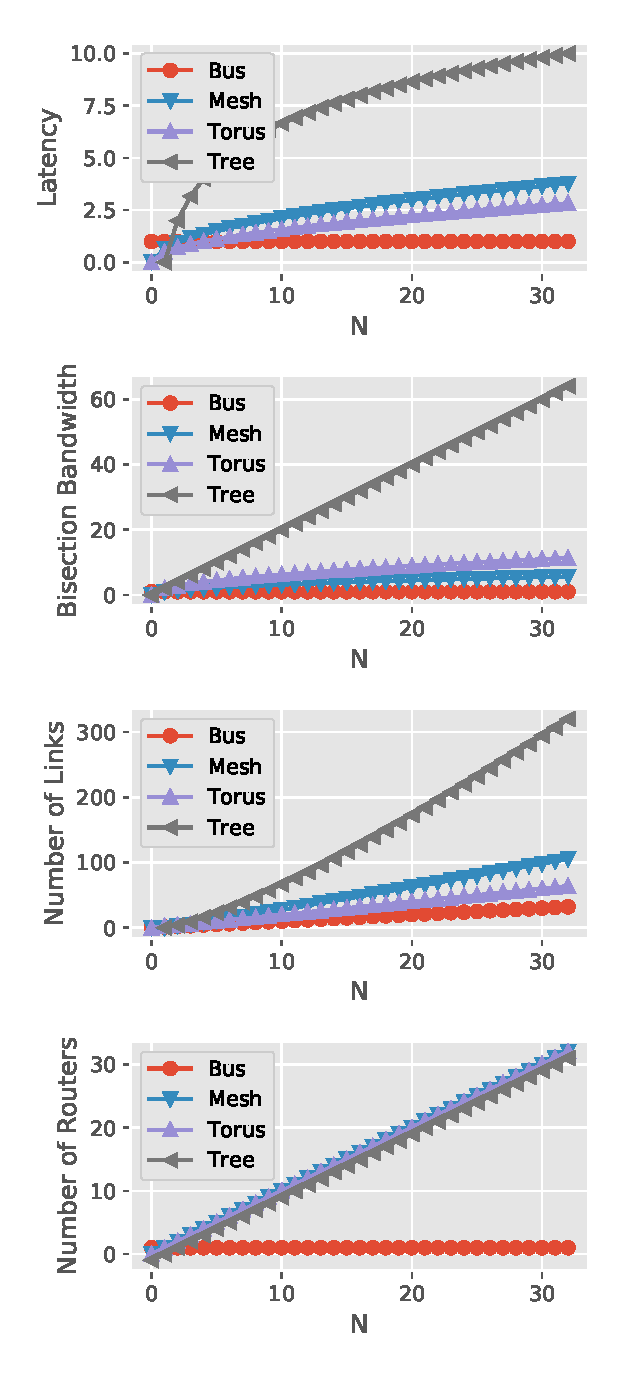
\includegraphics[width = 250pt]{expectations.eps}
    \caption{Expected latency relation for the four interconnect topologies derived from average distance}
    \label{fig:lat}
\end{figure}

\begin{figure*}
    \centering
        \begin{subfigure}[b]{.475\textwidth}
            \centering
            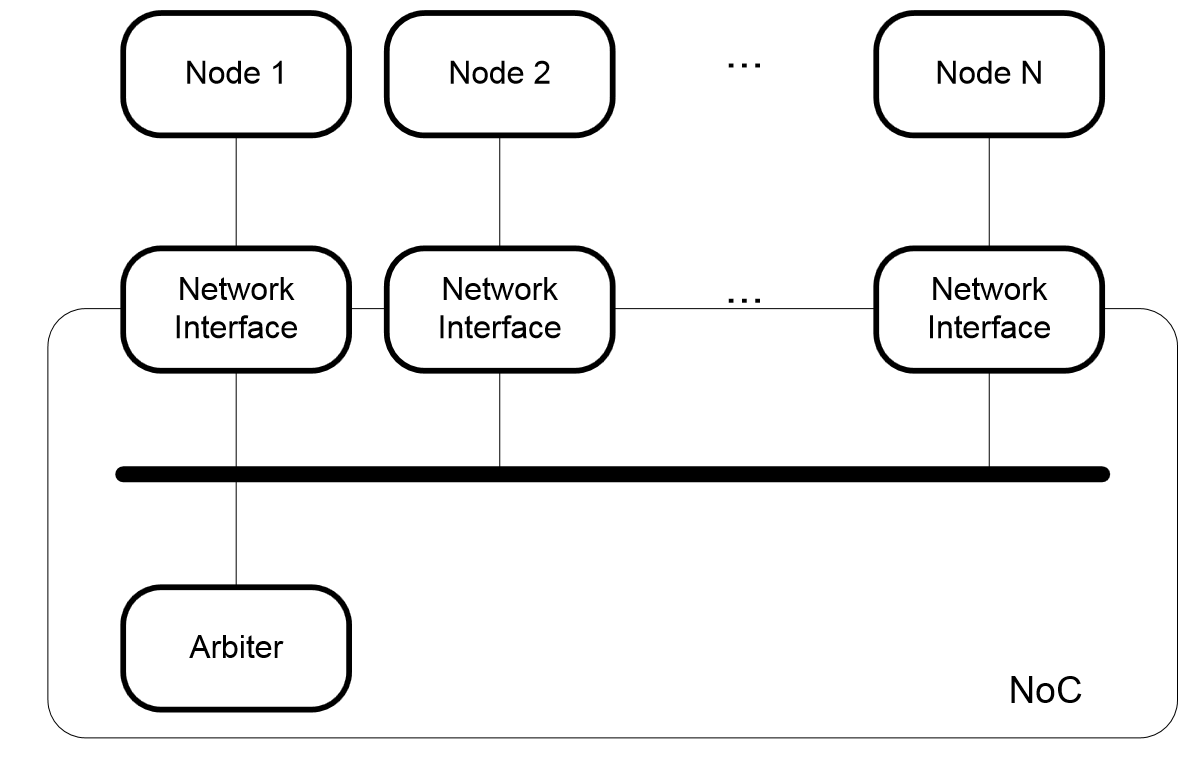
\includegraphics[width=\textwidth]{bus.png}
            \caption[]%
            {{\small }}    
            \label{ov1}
        \end{subfigure}
        \hfill
        \begin{subfigure}[b]{.475\textwidth}  
            \centering 
            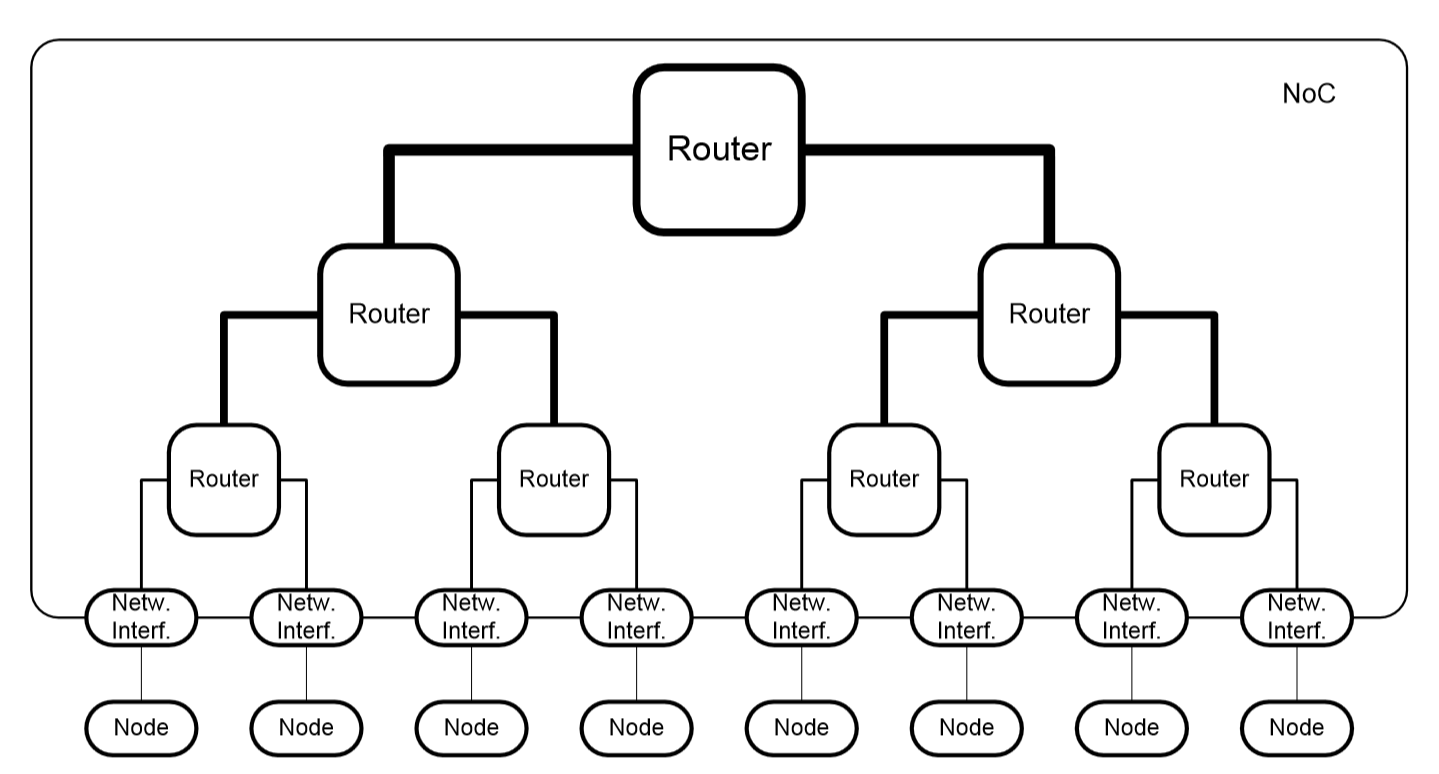
\includegraphics[width=\textwidth]{tree.png}
            \caption[]%
            {{\small }}    
            \label{ov2}
        \end{subfigure}
        \vskip\baselineskip
        \hfill
        \begin{subfigure}[b]{.475\textwidth}  
            \centering 
            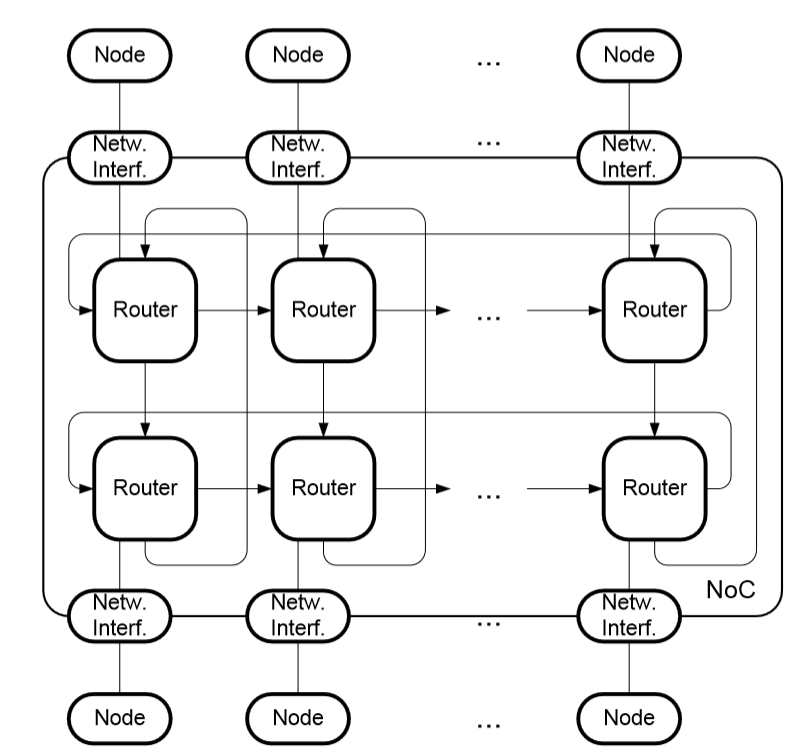
\includegraphics[width=\textwidth]{torus.png}
            \caption[]%
            {{\small }}    
            \label{ov2}
        \end{subfigure}
        \hfill
        \begin{subfigure}[b]{.475\textwidth}  
            \centering 
            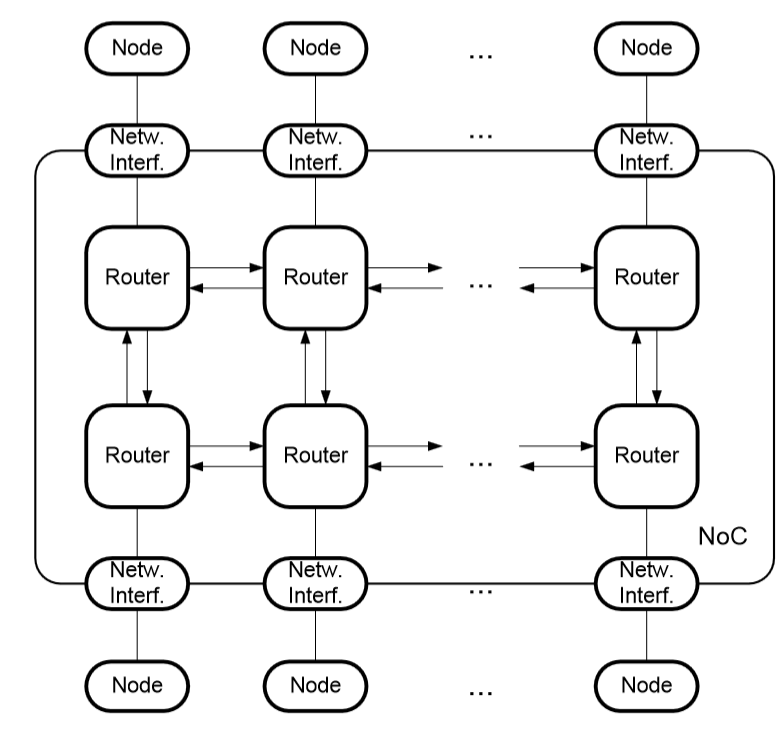
\includegraphics[width=\textwidth]{mesh.png}
            \caption[]%
            {{\small }}    
            \label{ov2}
        \end{subfigure}

        
        \caption[ The average and standard deviation of critical parameters ]
        {\small Illustration of the interconnect topologies a) Bus,b) Mesh, c) Torus, d) Fat tree} 
        \label{fig:illustration}
\end{figure*}

\section{Hypothesis}

Estimates of performance and scalabilty can generally be made by analysing the processor interconnect topologies. The average distance between nodes can be used to as an indication of the latency. Furthermore, an expectation of the available bandwidth for the nodes is made from the bisection bandwidth. This bisection bandwidth is determined by ... Besides performance also the cost and energy consumption are relevant metrics for a multiprocessor configuration. These metrics can be estimated by looking at the number of links and router that are required to realise a system with a certain number of nodes.      

\subsection{Bus}
Fig .. depicts the bus topology. This simple topology only requires on link per node and a single router (the arbiter). The performance of the bus may be sufficient for smaller number of nodes, however the bandwidth will not grow for a higher number of nodes (bisection bandwidth = 1). Therefore, high traffic with larger number of nodes will cause lots of blocking and therefore the scalability is expected to be very limited. The average distance between nodes does not necessarily grow as nodes are added to the system. Therefore, assuming low traffic a constant latency independent of to the number of nodes is expected.
\subsection{Mesh}
Figure \ref{fig:illustration} d depicts a mesh processor interconnect topology where nodes are positioned in a grid like fashion. In a mesh based system the average distance and bisection bandwidth scale better as the number of nodes grow. Therefore, the expected bandwidth is expected scale better with a larger number of nodes. However, this improvement of performance comes at a cost of more links and routers as evident from figure \ref{fig:num_routers} and \ref{fig:num_links}.  

\subsection{Torus}
For the unidirectional torus the latency per node is expected to be equal since all nodes have an equal amount of nodes to the right and below them. The average distance to a node is  


\subsection{Fat Tree}
The final topology discussed in this work is the Fat tree topology. For system with a large number of cores the fat tree topology provides the highest bandwidth. However, this does come at a significant cost in latency. Therefore, the tree topology might be a good solution when the frequency of the communication is low but a large amount of data needs to be transported.

\section{Simulation}

The analytical expressions used to generate a hypothesis are remain incomplete estimates the reality since they don't model how the network will  be affected by traffic. In practice, the scaleability of these networks may be determined by its capacity to handle dense traffic.    

Therefore, simulations are required in order to make accurate statements about the performance of the interconnect topologies. High level models of the interconnected processors can be made using the Poosl verification language. In these models a routing strategy can implemented such that the networks capacity for handling traffic can be evaluated. The simulations will assume that every node sends an equal amount of traffic and that the destinations for this traffic are equally distributed. To support the model several automation scripts in Python are used conveniently simulate the models for a varying amount of nodes. 

\subsection{Routing strategy}

The routing strategy employed for a network will affect the performance. Therefore, people commonly suggest adaptive routing strategies. However, for this work static routing strategies will be employed to keep the models manageable.

For the bus topology a round robin policy is used for routing. Meaning that every node gets equal sending time and that there are no live locks and deadlocks. 

The mesh interconnect model uses turn order routing which ensures no deadlocks or livelocks. Turn order routing ensures flits travel in the positive x/y direction before they start traveling in the negative y direction. 

For the mesh interconnect model a somewhat more complicated routing strategy is required due to the inherent cyclic dependencies, that can also be found in a ring interconnect system. This  With time domain multiplexing and using an extra queue for every link this problem can be resolved. In figure \ref{fig:cycDepend} the problem is illustrated, if all routers are occupied no packets can be transported and thus a deadlock emerges. However, by using virtual channels there will always be an escape somewhere and a deadlock will not emerge.

In order to apply this strategy from the ring to the two-dimensional torus it has to be extended in order to handle the extra dimension. This can be done use dimension order routing. This means that packets first travel to the x position of their destination before they travel to the y-position.  

\begin{figure}
    \centering
    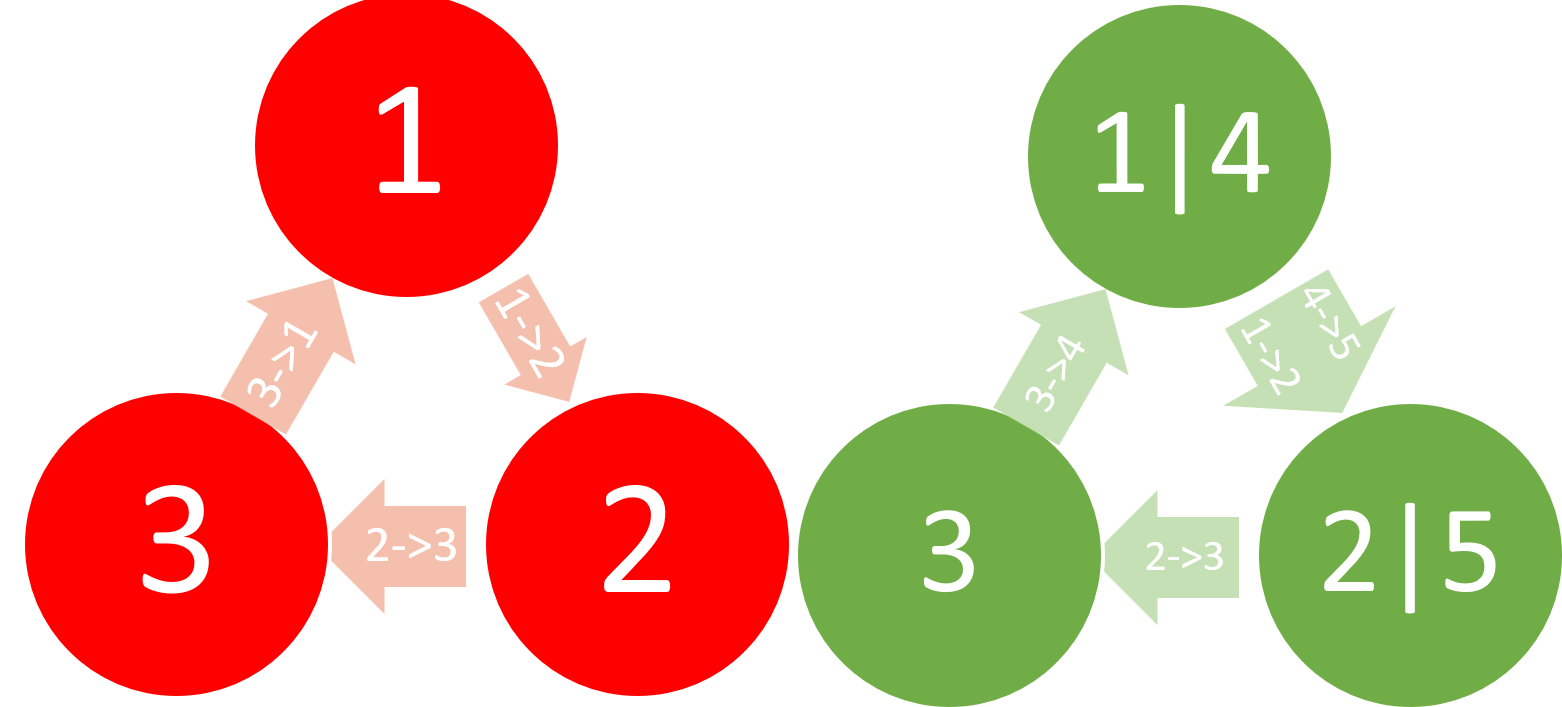
\includegraphics[width = 250pt]{cyclic.png}
    \caption{Cyclic dependencies and resolution with virtual channels}
    \label{fig:cycDepend}
\end{figure}



\section{Results}


\begin{figure*}
    \centering
        \begin{subfigure}[b]{.475\textwidth}
            \centering
            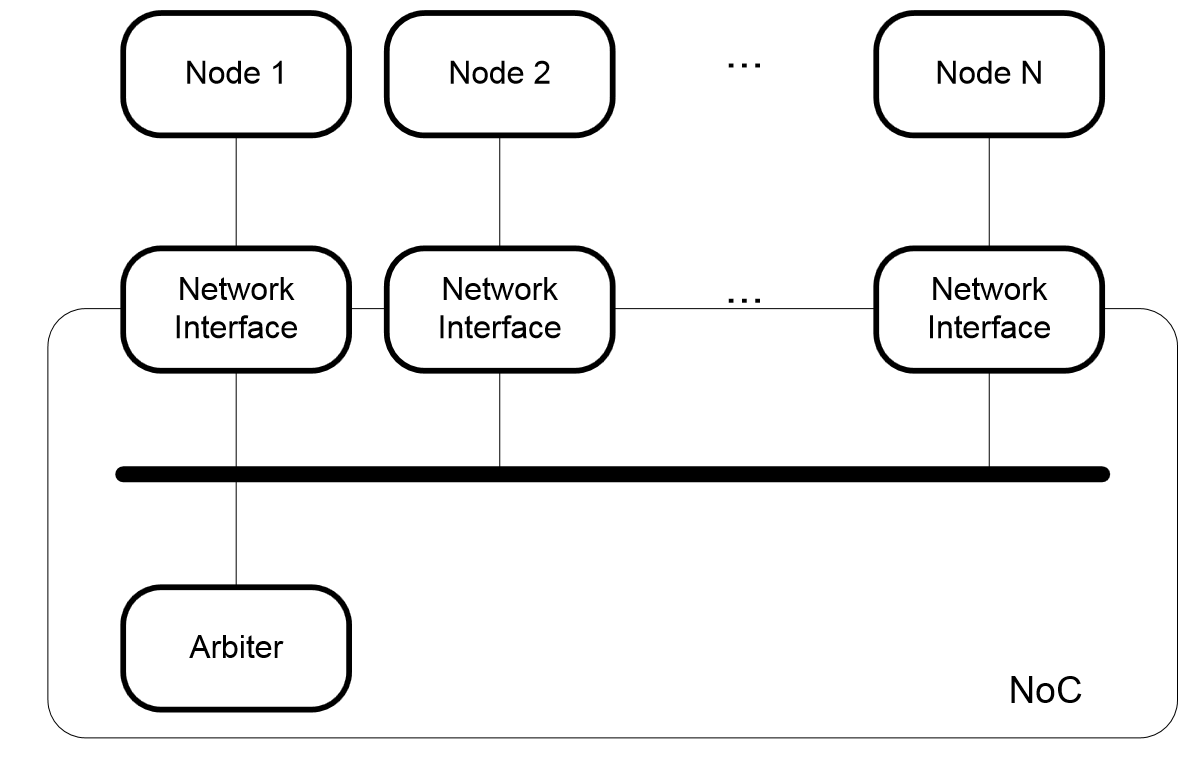
\includegraphics[width=\textwidth]{bus.png}
            \caption[]%
            {{\small }}    
            \label{ov1}
        \end{subfigure}
        \hfill
        \begin{subfigure}[b]{.475\textwidth}  
            \centering 
            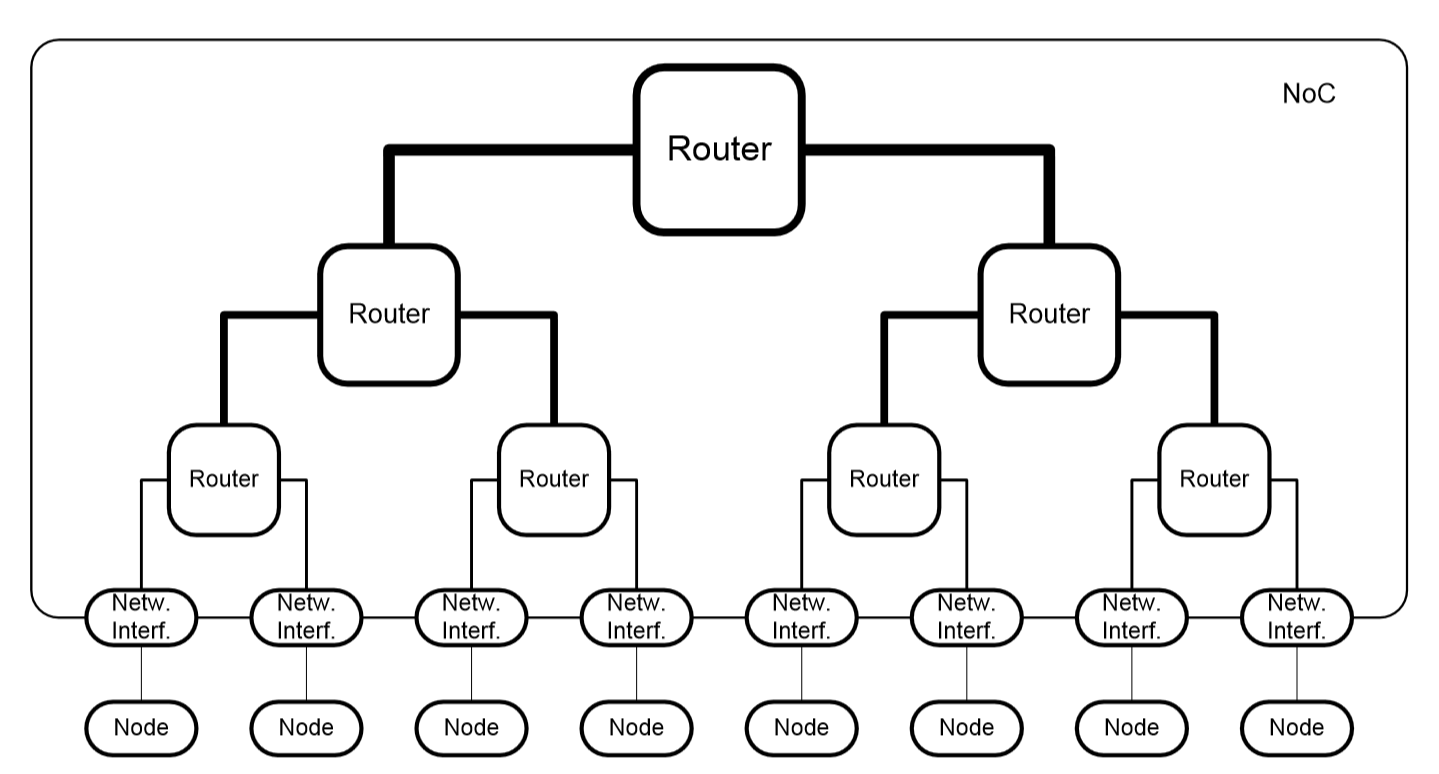
\includegraphics[width=\textwidth]{tree.png}
            \caption[]%
            {{\small }}    
            \label{ov2}
        \end{subfigure}
        \vskip\baselineskip
        \hfill
        \begin{subfigure}[b]{.475\textwidth}  
            \centering 
            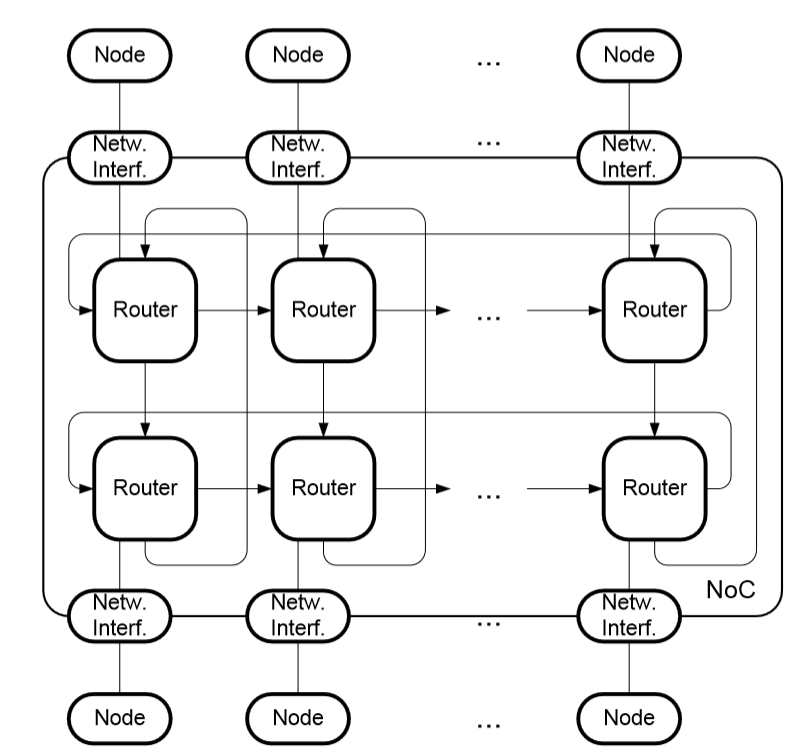
\includegraphics[width=\textwidth]{torus.png}
            \caption[]%
            {{\small }}    
            \label{ov2}
        \end{subfigure}
        \hfill
        \begin{subfigure}[b]{.475\textwidth}  
            \centering 
            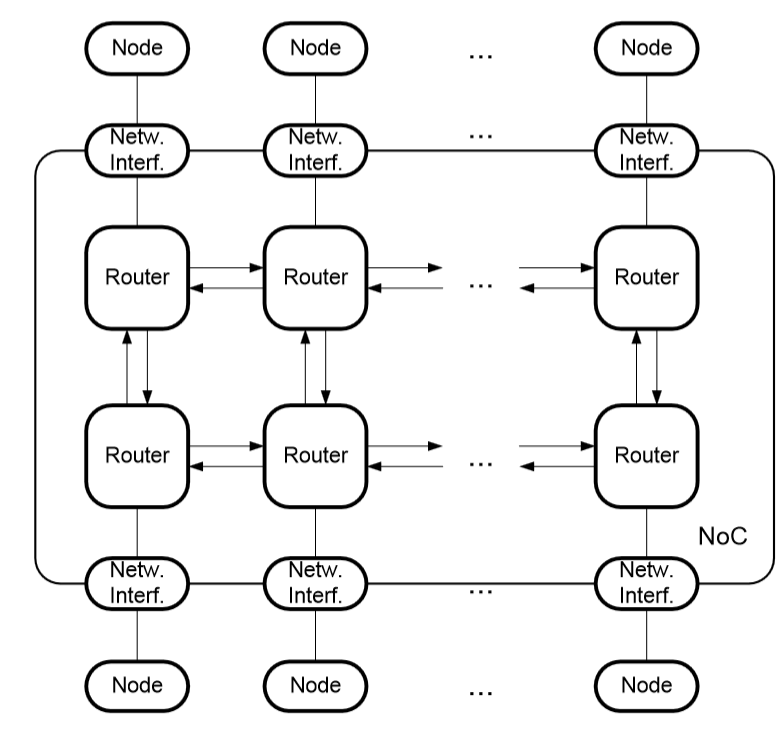
\includegraphics[width=\textwidth]{mesh.png}
            \caption[]%
            {{\small }}    
            \label{ov2}
        \end{subfigure}

        
        \caption[ The average and standard deviation of critical parameters ]
        {\small Illustration of the interconnect topologies a) Bus,b) Mesh, c) Torus, d) Fat tree} 
        \label{fig:illustration}
\end{figure*}


In fig ..  the results of the simulations have been depicted. Notably the torus performed not as well as expected initially however concidering the routing strategy required it quickly becomes obvious why its not so optimal. For both load values displayed in figure ...  the torus performs and scales badly.  




\end{document}